\documentclass[tikz,border=4pt]{standalone}
\usepackage{amsmath}
\begin{document}
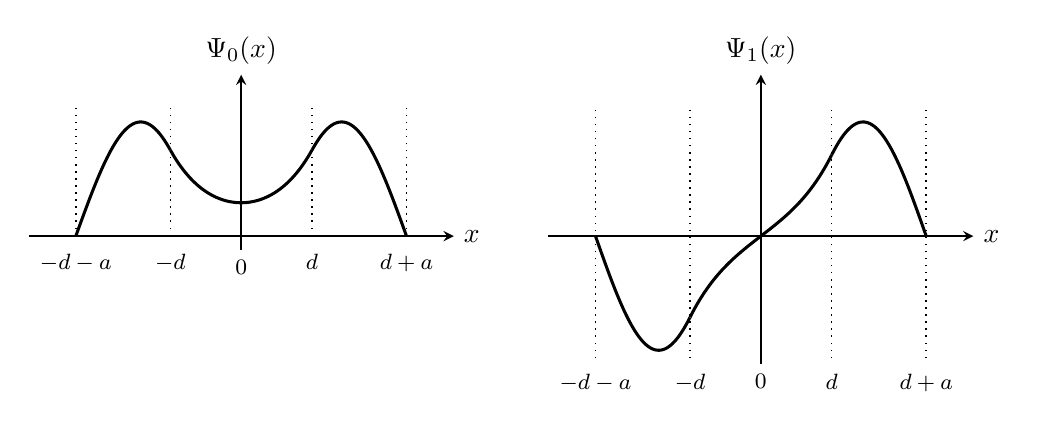
\begin{tikzpicture}[>=stealth, thick, scale=1.0]
  % Left panel: Ground state |Psi_0> (even parity)
  % Exact C^1-smooth parameters for a = 1.2, d = 0.9:
  % k0 = 1.906, kap0 = 1.78 => -k0*cot(1.2*k0) = 1.641 = kap0*tanh(0.9*kap0)
  % sin(1.906*1.2) = 0.7544; cosh(1.78*0.9) = 2.5825 => B0 = 1.45*0.7544/2.5825 = 0.4236
  \begin{scope}[xshift=0cm]
    \draw[->, line width=0.65pt] (-2.7, 0) -- (2.7, 0) node[right] {$x$};
    \draw[->, line width=0.65pt] (0, -0.18) -- (0, 2.05) node[above] {$\Psi_0(x)$};

    \foreach \xpos in {-2.1, -0.9, 0.9, 2.1} {
      \draw[dotted, line width=0.55pt] (\xpos, 0) -- (\xpos, 1.65);
    }
    \node[below, font=\footnotesize] at (-2.1, -0.10) {$-d-a$};
    \node[below, font=\footnotesize] at (-0.9, -0.10) {$-d$};
    \node[below, font=\footnotesize] at (0, -0.18) {$0$};
    \node[below, font=\footnotesize] at (0.9, -0.10) {$d$};
    \node[below, font=\footnotesize] at (2.1, -0.10) {$d+a$};

    \draw[line width=1.1pt, domain=-2.1:-0.9, samples=50, smooth] plot (\x, {1.45*sin(1.906*(2.1+\x) r)});
    \draw[line width=1.1pt, domain=-0.9:0.9, samples=50, smooth] plot (\x, {0.4236*cosh(1.78*\x)});
    \draw[line width=1.1pt, domain=0.9:2.1, samples=50, smooth] plot (\x, {1.45*sin(1.906*(2.1-\x) r)});
  \end{scope}

  % Right panel: First excited state |Psi_1> (odd parity)
  % Exact C^1-smooth parameters for a = 1.2, d = 0.9:
  % k1 = 1.958, kap1 = 1.78 => -k1*cot(1.2*k1) = 1.930 = kap1*coth(0.9*kap1)
  % sin(1.958*1.2) = 0.7117; sinh(1.78*0.9) = 2.3811 => B1 = 1.45*0.7117/2.3811 = 0.4334
  \begin{scope}[xshift=6.6cm]
    \draw[->, line width=0.65pt] (-2.7, 0) -- (2.7, 0) node[right] {$x$};
    \draw[->, line width=0.65pt] (0, -1.62) -- (0, 2.05) node[above] {$\Psi_1(x)$};

    \foreach \xpos in {-2.1, -0.9, 0.9, 2.1} {
      \draw[dotted, line width=0.55pt] (\xpos, -1.55) -- (\xpos, 1.65);
    }
    \node[below, font=\footnotesize] at (-2.1, -1.62) {$-d-a$};
    \node[below, font=\footnotesize] at (-0.9, -1.62) {$-d$};
    \node[below, font=\footnotesize] at (0, -1.62) {$0$};
    \node[below, font=\footnotesize] at (0.9, -1.62) {$d$};
    \node[below, font=\footnotesize] at (2.1, -1.62) {$d+a$};

    \draw[line width=1.1pt, domain=-2.1:-0.9, samples=50, smooth] plot (\x, {-1.45*sin(1.958*(2.1+\x) r)});
    \draw[line width=1.1pt, domain=-0.9:0.9, samples=50, smooth] plot (\x, {0.4334*sinh(1.78*\x)});
    \draw[line width=1.1pt, domain=0.9:2.1, samples=50, smooth] plot (\x, {1.45*sin(1.958*(2.1-\x) r)});
  \end{scope}
\end{tikzpicture}
\end{document}
